\documentclass[11pt, oneside]{article}   	% use "amsart" instead of "article" for AMSLaTeX format
\usepackage{geometry}                		% See geometry.pdf to learn the layout options. There are lots.
\geometry{letterpaper}                   		% ... or a4paper or a5paper or ... 
%\geometry{landscape}                		% Activate for rotated page geometry
%\usepackage[parfill]{parskip}    		% Activate to begin paragraphs with an empty line rather than an indent
\usepackage{graphicx}				% Use pdf, png, jpg, or eps§ with pdflatex; use eps in DVI mode
								% TeX will automatically convert eps --> pdf in pdflatex		
\usepackage{amssymb}

%SetFonts

%SetFonts


\title{Brief Article}
\author{The Author}
%\date{}							% Activate to display a given date or no date

\begin{document}
%\maketitle
%\section{}
%\subsection{}
\begin{flushright}
Donovan Guelde\\
CSCI 5622\\
SVM HW\\
\end{flushright}
\indent The Sklearn implementation of SVM was used to differentiate between 3's and 8's in the MNIST data set.  In an effort to get the highest accuracy, I implemented the linear, poly, and rbf kernel, each with a range of C values.\\
\\
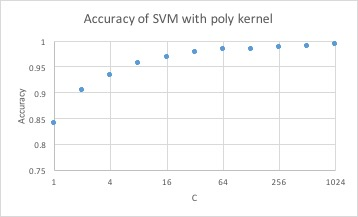
\includegraphics[width= .3\textwidth]{poly}
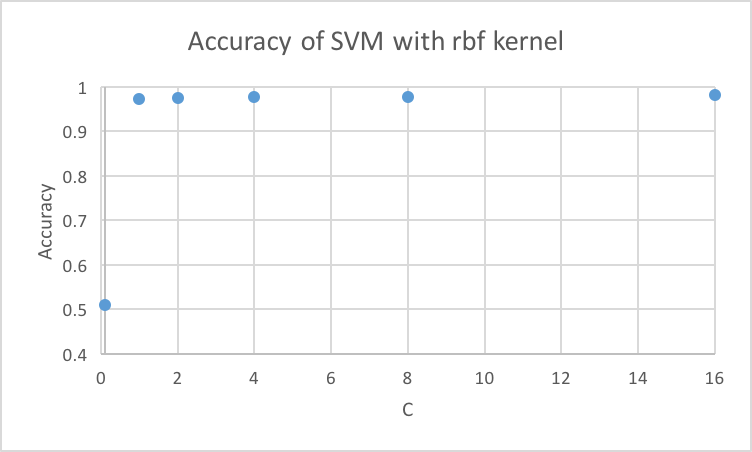
\includegraphics[width=.3\textwidth]{rbf}
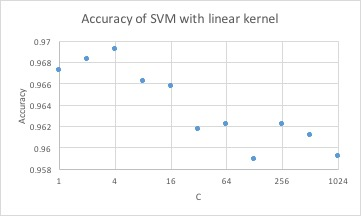
\includegraphics[width=.3\textwidth]{linear}\\
\\
\indent The poly kernel began to produce high accuracy with relatively small C values, even as low as $C = 2$, but maximum accuracy of 0.9929 was achieved on a test set at $C = 2048$.\\
\indent The rbf kernel produced accuracy of over .97 for all $C \geq 1$.  Where $C < 1$, accuracy drops drastically as $C$ approaches 0.  Maximum accuracy on the test set was 0.9914 at $C = 448$.\\
\indent The linear kernel produces reliably high accuracy for seemingly all C values, but never reaches the very high $(>.99)$ accuracy of the other two kernels.  This suggests that the data is nearly linearly seperable, with a handful of outliers.  Maximum accuracy for the linear kernel on the test set was 0.9698, with $C = 0.01$.  However, accuracy never dropped below .95 for any value of C.\\
\\

\includegraphics[width = .2\textwidth]{5}

\includegraphics[width = .2\textwidth]{4}
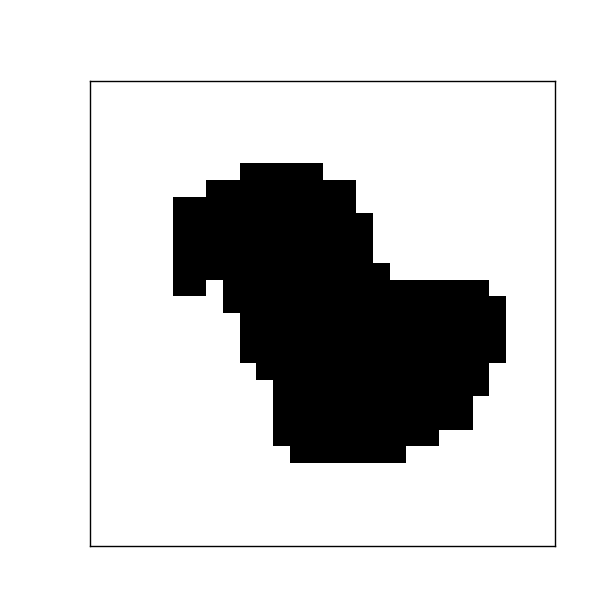
\includegraphics[width = .2\textwidth]{3}  Support vectors for class = 3
\\
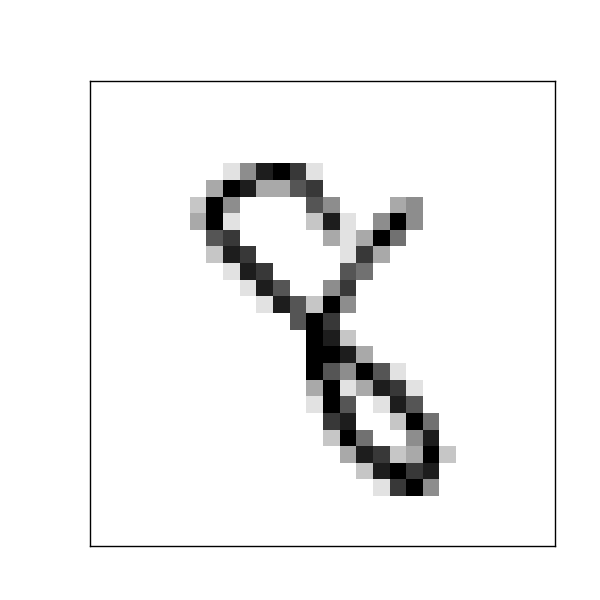
\includegraphics[width=.2\textwidth]{672}
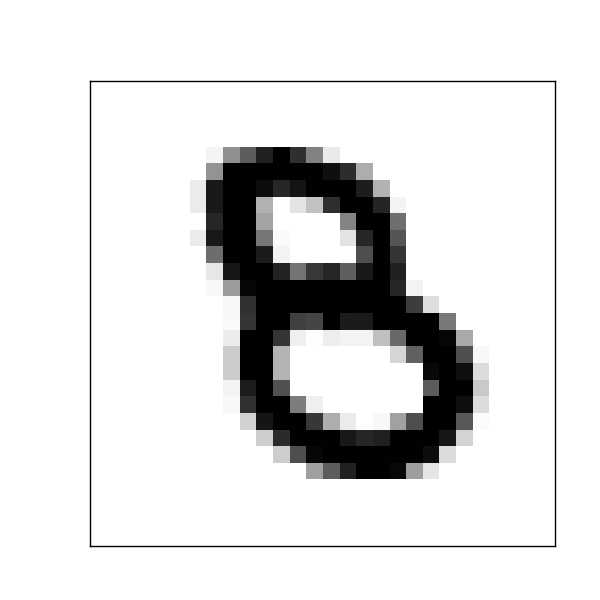
\includegraphics[width=.2\textwidth]{673}
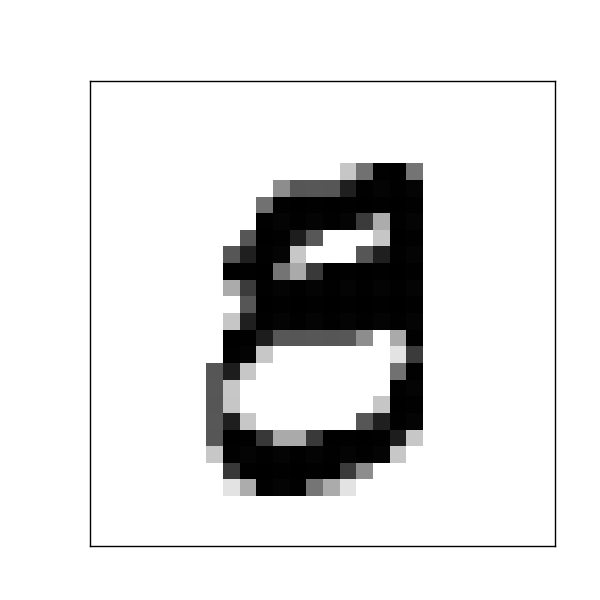
\includegraphics[width=.2\textwidth]{668}  Support vectors for class = 8
\\


\end{document}  